\section{Design}

In order to test SSO with OAuth and OIDC, we implement 3 applications with Django which is a high-level Python web framework that encourages rapid development and clean, pragmatic design. Django follows the model–template–views (MTV) architectural pattern. Django's primary goal is to ease the creation of complex, database-driven websites. The framework emphasizes reusability and "pluggability" of components, less code, low coupling, rapid development, and the principle of don't repeat yourself. Python is used throughout, even for settings, files, and data models. Django also provides an optional administrative create, read, update and delete interface that is generated dynamically through introspection and configured via admin models.

   

\subsection*{3.1 OAuth 2.0}

OAuth 2.0 is an open-standard authorization protocol that provides applications the ability for “secure designated access.” For example, you can tell Facebook that it’s OK for YouTube.com to access your profile or post updates to your timeline without having to give YouTube your Facebook password. This minimizes risk in a major way: In the event YouTube suffers a breach, your Facebook password remains safe.


Glossary of the components are, \textbf{a) Resource Owner} the user, \textbf{b) Resource Server} a service hosting data, \textbf{c) Client} an application that accesses data residing the resource server, \textbf{d) Authorization Server} authenticates the user and grants tokens, \textbf{e) Access Token} a piece of data that represents the authorization to access resources on behalf of the resource owner.


To enable the OAuth protocol in our project we need to create the \textbf{Provider}, acting both as Resource Server and Authorization Server, (Resource Server and Authorization Server can be separate applications, for this project it's the same) and the \textbf{Client}.
For implementing the Provider we used \textbf{Django OAuth Toolkit} package, which provides all the endpoints, data, and logic needed to add OAuth 2.0 capabilities to our Django project.
With the toolkit we made our own Authorization Server to issue access tokens to Client applications for a certain API, all we need to do is to include (vale kwdika) to installed apps and add the urls that toolkit provides by adding  \textbf{vazw codika edw ?} in url patterns. Now the provider knows where to look for the endpoints that the toolkit provides.

Before our Application (the Client), can use the Authorization Server for (???OAuth capabilities??????) user login, we must first register the app. Once registered, the Client will be granted access to the API, subject to approval by its users. The registration process will automatically generate a unique Client\_id and Client\_secret, which are used so the Client and the Authorization Server establish a working relationship. The Authorization Server generated the Client ID and Client Secret, sometimes called the App ID and App Secret, and gave them to the Client to use for all future OAuth exchanges. Client Secret must be kept secret so that only the Client and Authorization Server know what it is. This is how the Authorization Server can verify the Client. We have to provide the rest of the informations:

\begin{description}
	
	\item[$\bullet$ User:] the owner of the Application (e.g. a developer, or the currently logged in user.)
	
	\item[$\bullet$ Redirect uris:]Applications must register at least one redirection endpoint before using the authorization endpoint. The Authorization Server will deliver the access token to the client only if the client specifies one of the verified redirection uris.
	
	\item[$\bullet$ Client type:] this value affects the security level at which some communications between the client application and the authorization server are performed. For this project we use Confidential.
	
	\item[$\bullet$ Authorization grant type:] Authorization code
	
	\item[$\bullet$ Name:] this is the name of the client application on the server, and will be displayed on the authorization request page, where users can allow/deny access to their data.
	
\end{description}

We used Authorization code grant type, because authorizing an application to access OAuth protected data, with this grant type, flow is always initiated by the user and application can prompt users to click a special link to start the process. When a user clicks the link, user is redirected to Authorization Server.  If user is not logged in, he will be prompted for username and password. This is because the authorization page is login protected by django-oauth-toolkit. Login, then should see the form a user can use to give his authorization to the client application. User flags the checkbox, click Authorize, and he will be redirected again to the client.

At this point the Authorization Server redirected the user to a special page on the Client passing in an Authorization Code, a special token the Client will use to obtain the final Access Token. This operation is usually done automatically by the Client application during the request/response cycle. Access Tokens has a specific lifetime, given by the Authorization Server. For that case the Access Token has a Refresh Token aswell and it's used for a brand new access token, without repeating the authorization process, it has no expire time.


\definecolor{OAUTH}{RGB}{0 0 0}
\begin{center}
	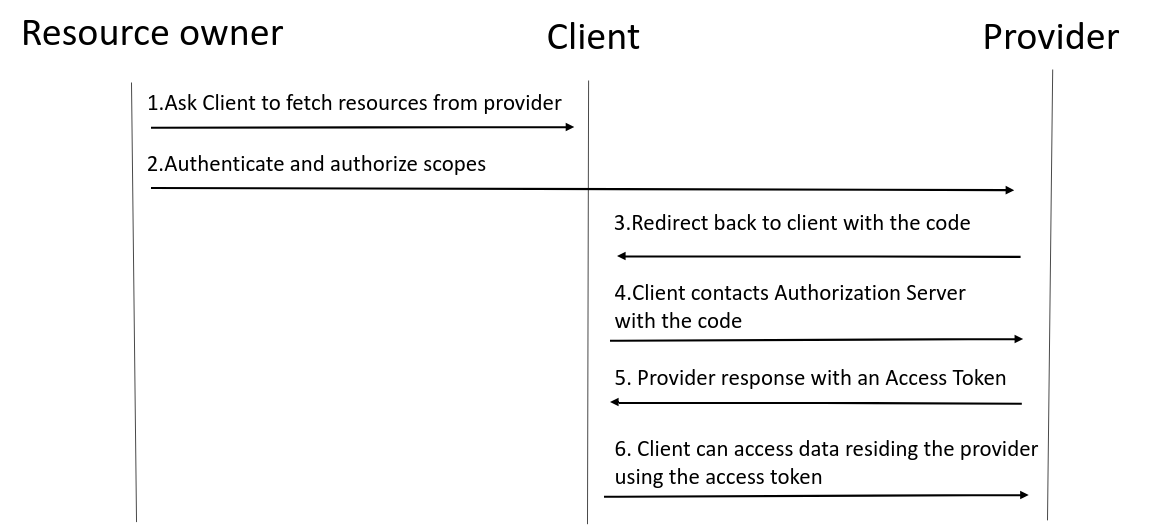
\includegraphics[scale=0.3]{figures/oauth.png}\\
	\textcolor{OAUTH}{\textbf{3.2 OAuth flow}}
\end{center}


\subsection*{3.3 OpenID Connect}

OAuth 2.0 is designed only for authorization, for granting access to data and features from one application to another. OpenID Connect (OIDC) is a thin layer that sits on top of OAuth 2.0 that adds login and profile information about the person who is logged in. Establishing a login session is often referred to as authentication, and information about the person logged in (i.e. the Resource Owner) is called identity. When an Authorization Server supports OIDC, it is sometimes called an identity provider, since it provides information about the Resource Owner back to the Client. OIDC flow looks the same as OAuth, the only differences are, in the initial request, a specific scope of \textbf{openid} is used, and the Server responds with an Access Token and A JSON Web Token (JWT) that contains the information about the Resource owner.


\definecolor{OIDC}{RGB}{0 0 0}
\begin{center}
	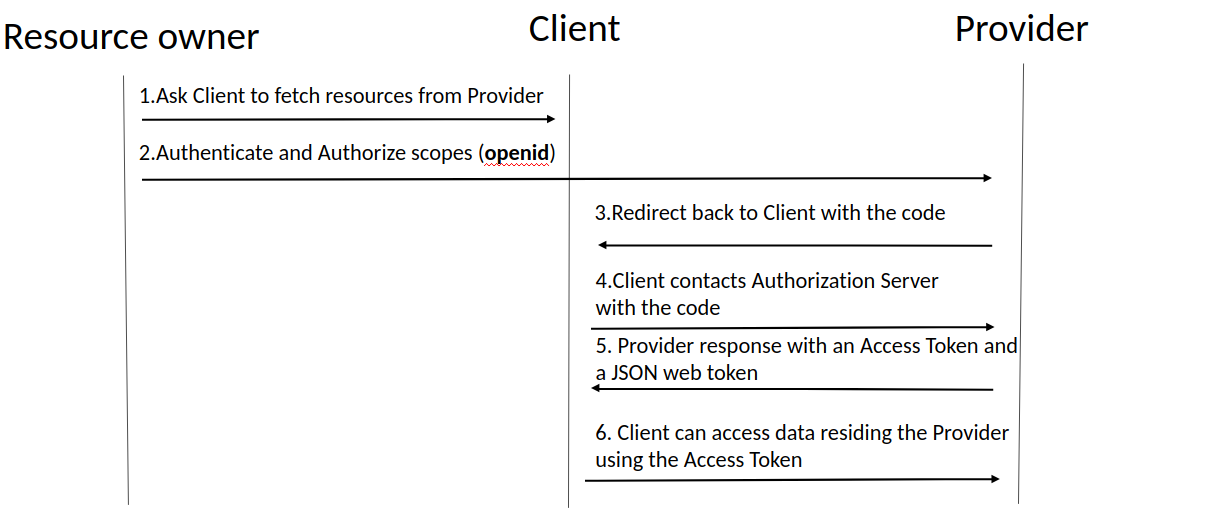
\includegraphics[scale=0.4]{figures/OIDC.png}\\
	\textcolor{OIDC}{\textbf{3.4 OIDC flow}}
	
\end{center}


\subsection*{3.5 Lightweight Directory Access Protocol}

The Lightweight Directory Access Protocol (LDAP) is one of the core authentication protocols that was developed for directory services. LDAP historically has been used as a database of information, primarily storing information like \textbf{users}, \textbf{Attributes about those users}, \textbf{group membership privileges} and more. This information was then used to enable authentication to IT resources such as an application or server. They would be pointed to the LDAP database, which would then validate whether that user would have access to it or not. That validation would be done passing a user’s credentials. LDAP authentication follows the client/server model. In this scenario, the client is generally an LDAP-ready system or application that is requesting information from an associated LDAP database and the server is, of course, the LDAP server. The server side of LDAP is a database that has a flexible schema. In other words, not only can LDAP store username and password information, but it can also store a variety of attributes including address, telephone number, group associations, and more. As a result, a common LDAP use case is to store core user identities. In doing so, IT can point LDAP-enabled systems and applications (for example) to an associated LDAP directory database, which acts as the source of truth for authenticating user access. 


We add LDAP authentication in OIDC Provider using \textbf{auth-ldap} package. This package  is a Django authentication backend that authenticates against an LDAP service (in this case FORTH'S LDAP Server). Configuration can be as simple as a single distinguished name template, but there are many rich configuration options for working with users, groups, and permissions. For authentication with the LDAP server we need to follow these steps : 

\begin{description}
	\item[$\bullet$] Add 'django\_auth\_ldap.backend.LDAPBackend' to AUTHENTICATION\_BACKENDS
	\item[$\bullet$] Set AUTH\_LDAP\_SERVER\_URI to point the LDAP Server
\end{description}

Now that we can talk to LDAP server, the next step is to authenticate a username and password. There are two ways to do this, called \textbf{search/bind} and \textbf{direct bind}. The first one involves connecting to the LDAP server either anonymously or with a fixed account and searching for the distinguished name of the authenticating user. Then we can attempt to bind again with the user’s password. The second method is to derive the user’s DN from his username and attempt to bind as the user directly.

We used Direct Bind, to skip the search phase, all we need to do is to set AUTH\_LDAP\_USER\_DN\_TEMPLATE to a template that will produce the authenticating user’s DN directly. This template should have one placeholder, \%(user)s. By setting AUTH\_LDAP\_USER\_ATTR\_MAP we are able to match our user's model attributes with the ldap user. 
With these settings we are able to connect to a LDAP server. When the LDAP authenticates the users credentials, the auth-ldap backend will return a ldap\_user and will create a django user to return and create with the attributes that we gave before. 


\definecolor{LDAP}{RGB}{0 0 0}
\begin{center}
	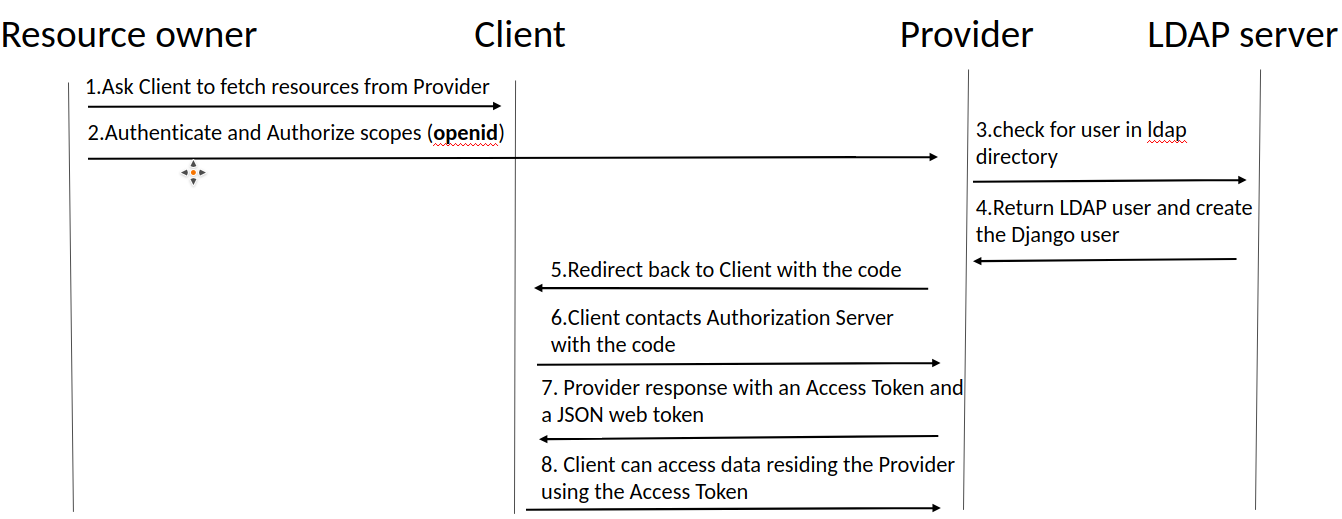
\includegraphics[scale=0.4]{figures/LDAP.png}\\
	\textcolor{LDAP}{\textbf{3.4 OIDC with LDAP flow}}
\end{center}
 



























